\documentclass[12pt,a4paper,twoside]{article}
\usepackage[utf8]{inputenc}
\usepackage{amsmath,amsfonts,amssymb}
\usepackage{float}
\usepackage{caption}
\usepackage{booktabs}
\usepackage{pgfplots}
\pgfplotsset{compat=1.18}
\usepackage{tikz}
\usetikzlibrary{calc,angles,quotes}
\usepackage{adjustbox}
\usepackage{array}
\usepackage{multirow}
\usepackage{longtable}
\usepackage{tabularx}
\usepackage{siunitx}
\usepackage{microtype}
\usepackage{multicol}
\usepackage{listings}
\usepackage{xcolor}
\usepackage[hidelinks]{hyperref}
\usepackage[a4paper]{geometry}
\usepackage[utf8]{inputenc}
\geometry{
  top=1 in,
  bottom=1 in,
  inner=1.25 in,   
  outer=1 in       
}

\usepackage{graphicx}

\begin{document}

\begin{titlepage}

\centering

\begin{flushleft}
    \includegraphics[width=0.18\textwidth]{footer-logo.png}
\end{flushleft}

\vspace{1cm}

{\Large \textbf{Mohamed El Bachir El Ibrahimi University of Bordj Bou Arréridj} \par}

{\large Faculty of Science and Technology \par}

{\large Department of Materials Science \par}

{\large Undergraduate Programme (LMD) – Physics – Year 2\par}
   
{\large Course: Geometrical and Physical Optics\par}
   

\vspace*{\fill}
{\Huge \textbf{Practical Work  N\textsuperscript{o}:1} \\ Experimental Verification of the Laws of Reflection and Refraction on a Plane Diopter \par}
\vspace*{\fill}

  {\large \textbf{Submitted by:} \\
Mezhoud maroua \par}

\vspace{1 cm}
    
    {\large \textbf{Supervised by:} \\ Dr. S. Mameri\par}
  
\vspace{2 cm}
    
    {\large Date of submission: November 11, 2025 \par}
   
    {\large Academic Year: 2025–2026 \par}  
    
\vfill
    
\end{titlepage}

\pagenumbering{Roman}  

\pagestyle{plain}

\begin{abstract}
This experiment aimed to verify Snell’s and Descartes’ laws of reflection and refraction using a plane diopter and a plane mirror. 
Angles of incidence, reflection, and refraction were measured for several light rays, and the relationship between $\sin(i)$ and $\sin(r)$ was analyzed. 
The results showed that the angle of reflection closely matches the angle of incidence within the experimental uncertainty ($\pm 0.1^\circ$), and that $\sin(i)$ and $\sin(r)$ are linearly related, in full agreement with Snell’s law. 
From the slope of the linear fit, the refractive index of the transparent medium was determined to be $n = 1.39 \pm 0.06$. 
The material used was a transparent polymer, PMMA, with optical properties similar to glass. 
These results confirm the validity of the laws of reflection and refraction, demonstrate the precision and reliability of the experimental procedure, and illustrate that transparent thermoplastic polymers can effectively be used for laboratory studies of optical phenomena.
\end{abstract}

\tableofcontents

\newpage 

\pagenumbering{arabic}  
\setcounter{page}{1}  

\section{Introduction} 

When light passes from one medium to another with different optical properties, it undergoes phenomena such as reflection and refraction, described by Snell’s and Descartes’ laws.  
Verifying these fundamental laws provides deeper insight into the behavior of light at an interface and enables the determination of key optical parameters, such as the refractive index of materials.  
In this experiment, the reflection and refraction of light on a plane diopter and a plane mirror were investigated to verify these laws experimentally and to compare the measured results with theoretical predictions.

\section{Objective}
The objectives of this experiment are to:
\begin{itemize}
  \item Experimentally verify Snell's and Descartes' laws of reflection and refraction.
  \item Determine the refractive index of the transparent medium used.
\end{itemize}

\section{Theoretical Background}

\subsection{Reflection of Light}
When a light ray strikes a reflecting surface, it bounces back into the same medium. This phenomenon is governed by \textbf{Descartes’ Law of Reflection}, which states:

\[
i = r
\]

Where: 
\begin{itemize}
    \item $i$ is the angle of incidence measured from the normal.
    \item $r$ is the angle of reflection measured from the normal.
\end{itemize}

\textbf{Key points:}
\begin{itemize}
    \item The incident ray, reflected ray, and the normal all lie in the same plane.
    \item This law applies to all types of reflective surfaces, whether plane or curved.
\end{itemize}

\begin{figure}[H]
\centering
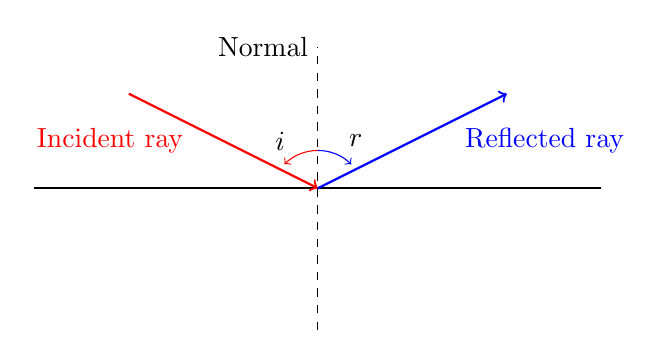
\begin{tikzpicture}[scale=1.2]
% Draw the surface
\draw[thick] (-3,0) -- (3,0);
% Draw normal
\draw[dashed] (0,-1.5) -- (0,1.5);
\node[left] at (0,1.5) {Normal};
% Incident ray
\draw[->, red, thick] (-2,1) -- (0,0) 
node at (-2.2,0.5) {Incident ray};
% Reflected ray
\draw[->, blue, thick] (0,0) -- (2,1) 
node at (2.4,0.5) {Reflected ray};
% Angle labels
\draw [->,red] (0,0.4) arc[start angle=90,end angle=135,radius=0.5cm];
\node at (-0.4,0.5) {$i$};
\draw [->,blue] (0,0.4) arc[start angle=90,end angle=45,radius=0.5cm];
\node at (0.4,0.5) {$r$};
\end{tikzpicture}
\caption{Reflection of light at a plane surface.}
\end{figure}

\subsection{Refraction of Light}
When a light ray passes from one transparent medium to another, its speed changes, causing the ray to bend. This is described by \textbf{Snell's Law}:

\[
n_1 \, \sin(i) = n_2 \, \sin(r)
\]

Where:
\begin{itemize}
    \item $n_1$ and $n_2$ are the refractive indices of the first and second media.
    \item $i$ is the angle of incidence.
    \item $r$ is the angle of refraction.
\end{itemize}

The refractive index $n$ of a medium is defined as:
\[
n = \frac{c}{v}
\]

Where \( c \) is the speed of light in vacuum (\( c \approx 3.00 \times 10^8 \, \text{m/s} \)), and \( v \) denotes the speed of light as it propagates through the medium.

\textbf{Key points:}
\begin{itemize}
    \item The incident ray, refracted ray, and normal lie in the same plane.
    \item Light bends \textbf{toward the normal} when it enters a denser medium ($n_2 > n_1$) and \textbf{away from the normal} when entering a less dense medium ($n_2 < n_1$).
\end{itemize}

\begin{figure}[H]
\centering
\begin{tikzpicture}[scale=1.5]
% --- Media regions ---
\fill[blue!10] (-3,-2) rectangle (3,0); % Denser medium (glass)
\fill[white] (-3,0) rectangle (3,2);    % Rarer medium (air)
\draw[thick] (-3,0) -- (3,0);           % Boundary line
% --- Normal ---
\draw[dashed] (0,2) -- (0,-2);
\node at (-0.6,1.9) {Normal};
% --- Incident ray ---
\draw[->, red, thick] (-2,1.3) -- (0,0)
    node at (-2,0.7) {Incident ray};
    
% --- Refracted ray (bends toward normal) ---
\draw[dashed] (0,0) -- (2,-1.3)

\draw[->, green!60!black, thick] (0,0) -- (0.8,-1)
    node at (1.6,-0.7) {Refracted ray};
    
% --- Angle of incidence ---
\draw[->, thin] (0,0.4) arc[start angle=90,end angle=132,radius=0.4cm];
\node at (-0.2,0.5) {$i$};
% --- Angle of refraction (smaller) ---
\draw[->, thin] (0,-0.4) arc[start angle=250,end angle=290,radius=0.4cm];
\node at (0.2,-0.6) {$r$};
% --- Labels for media ---
\node[font=\small] at (1.8,1) {Air ($n_1$)};
\node[font=\small] at (1.8,-1.5) {($n_2 > n_1$)};
\end{tikzpicture}
\caption{Refraction of light at a plane diopter. The refracted ray bends toward the normal when entering a denser medium ($n_2 > n_1$).}
\label{fig:refraction_plane_diopter}
\end{figure}

\subsection{Graphical Representation and Experimental Determination of $n$}

For a plane diopter, Snell's law predicts that a plot of $\sin(i)$ versus $\sin(r)$ should yield a straight line passing through the origin:

\begin{equation}
\sin(r) = a \, \sin(i)
\end{equation}

\noindent where
\[
a = \frac{n_1}{n_2},
\]
and \(n_1 \approx 1.0003\) for air (often approximated as \(n_1 \simeq 1\)).


From the slope $a$ of the experimental plot, the refractive index $n_2$ of the medium can be determined as:
\[
n_2 = \frac{1}{a}.
\]

\section{Apparatus and Materials}

The following apparatus and materials were used in the experiment:

\begin{itemize}
   \item \textbf{Optical board} – flat base with an angular scale for precise alignment.
   \item \textbf{Light source} – produces a narrow and well-defined beam.
   \item \textbf{Plane transparent surface} – to observe and measure refraction angles.
   \item \textbf{Plane mirror} – to observe and measure reflection angles.
   \item \textbf{Ruler and pencil} – for accurately tracing the light rays.
\end{itemize}

\section{Experimental Procedure}

The experiment was carried out using an optical bench equipped with an angularly graduated disk.

\subsection*{Experiment 1: Refraction at a Plane Diopter}
A transparent rectangular block was placed at the center of the bench so that the normal to its surface coincided with the reference line at an angle of \(0^\circ\).  
This block acted as a \textbf{plane diopter} to study the phenomenon of refraction.

A narrow light beam emitted from a lamp was directed toward the refracting surface, and the angles of incidence \(i\) and refraction \(r\) were accurately measured.  
Each measurement was repeated three times (\(r_1, r_2, r_3\)), and the average value was calculated as:
\[
r_{\text{avg}} = \frac{r_1 + r_2 + r_3}{3}
\]
to reduce experimental errors.  
The procedure was repeated for several incidence angles ranging from \(0^\circ\) to \(80^\circ\), with a constant increment of \(5^\circ\) between successive measurements.

\subsection*{Experiment 2: Reflection on a Plane Mirror}
The plane interface was then replaced by a plane mirror to study the phenomenon of reflection.  
The light beam was directed toward the mirror surface, and the path of the reflected beam was traced for incidence angles between \(0^\circ\) and \(10^\circ\).  
Each angle was measured three times (\(i'_1, i'_2, i'_3\)), and the average value was calculated as:
\[
i'_{\text{avg}} = \frac{i'_1 + i'_2 + i'_3}{3}
\]
to ensure accuracy.  
The \textbf{law of reflection} was verified by comparing the measured incidence and reflection angles in each case.

\subsection*{General Remarks}
All measurements were performed under normal laboratory lighting conditions and at room temperature.  
Special care was taken to minimize \emph{parallax errors} and alignment inaccuracies during ray tracing and angle readings.

\textbf{As illustrated in the figure below:}

\begin{figure}[H]
\centering
\adjustbox{fbox=1pt,margin=0pt,bgcolor=white}{%
  \includegraphics[width=0.75\textwidth]{5766862084971891532.jpg}%
}
\caption{Experimental setup for the plane diopter.}
\label{fig:dioptre_plan_setup}
\end{figure}

\section{Results and Discussion}
In this section, we present and analyze the experimental results obtained for both the refraction at a plane diopter and the reflection on a plane mirror.
\subsection{Experiment 1: Refraction at a Plane Diopter}

The measurements of the angles of incidence, reflection, and refraction are summarized in Table \ref{tab:plane_diopter_corrected}.

\begin{center}
\resizebox{\textwidth}{!}{
\begin{tabular}{|c|*{17}{c|}}
\hline
\textbf{Angle of incidence} $i$ (\si{\degree}) 
& 0 & 5 & 10 & 15 & 20 & 25 & 30 & 35 & 40 & 45 & 50 & 55 & 60 & 65 & 70 & 75 & 80 \\
\hline
\textbf{Angle of reflection} $i'$ (\si{\degree}) 
& 0 & 5 & 10 & 15 & 20 & 25 & 30 & 35 & 40 & 45 & 50 & 55 & 60 & 65 & 70 & 75 & 80 \\
\hline
\textbf{Angle of refraction} $r_1$ (\si{\degree}) 
& 0 & 4 & 8.7 & 10 & 14 & 18 & 20.9 & 23.8 & 26.1 & 29.1 & 32 & 36.2 & 38 & 39 & 42.5 & 41 & 44 \\
\hline
\textbf{Angle of refraction} $r_2$ (\si{\degree}) 
& 0 & 4.5 & 8.5 & 11.5 & 14.2 & 19 & 21 & 24 & 26 & 29 & 32 & 36 & 38 & 39 & 40 & 42 & 43 \\
\hline
\textbf{Angle of refraction} $r_3$ (\si{\degree}) 
& 0 & 5 & 8 & 11 & 14.5 & 18.2 & 21.5 & 24.2 & 26.4 & 28.8 & 32 & 36.6 & 38.2 & 39 & 40.5 & 42 & 43.5 \\
\hline
\textbf{Angle of refraction} $r_{\mathrm{moy}}$ (\si{\degree}) 
& 0.00 & 4.50 & 8.40 & 10.83 & 14.23 & 18.40 & 21.13 & 24.00 & 26.17 & 29.30 & 32.00 & 36.27 & 38.13 & 39.00 & 41.00 & 41.67 & 43.50 \\
\hline
$\boldsymbol{\sin(i)}$ 
& 0.000 & 0.087 & 0.174 & 0.259 & 0.342 & 0.423 & 0.500 & 0.574 & 0.643 & 0.707 & 0.766 & 0.819 & 0.866 & 0.906 & 0.940 & 0.966 & 0.985 \\
\hline
$\boldsymbol{\sin(r_{\mathrm{moy}})}$ 
& 0.000 & 0.078 & 0.146 & 0.188 & 0.246 & 0.316 & 0.360 & 0.406 & 0.441 & 0.489 & 0.530 & 0.593 & 0.617 & 0.629 & 0.656 & 0.666 & 0.688 \\
\hline
\end{tabular}
}
\vspace{0.5 cm}
\captionof{table}{Experimental measurements for the plane diopter}
\label{tab:plane_diopter_corrected}
\end{center}

\begin{figure}[H]
\centering
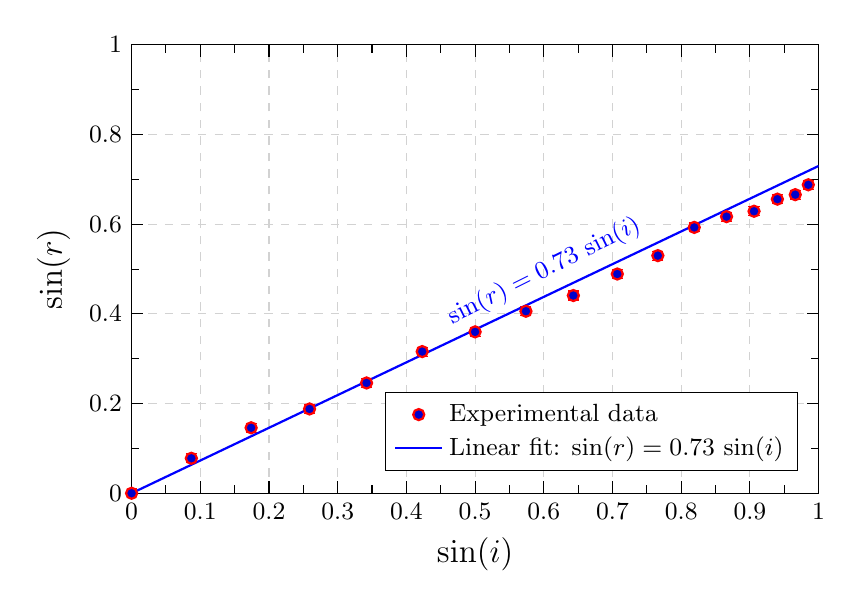
\begin{tikzpicture}
\begin{axis}[
    width=0.85\textwidth,
    height=0.6\textwidth,
    xlabel={$\sin(i)$},
    ylabel={$\sin(r)$},
    xmin=0, xmax=1,
    ymin=0, ymax=1,
    grid=major,
    grid style={gray!35, dashed},
    minor tick num=1,
    tick style={black, thin},
    label style={font=\large},
    tick label style={font=\small},
    legend style={font=\small, at={(0.97,0.05)}, anchor=south east, cells={anchor=west}},
    every axis plot/.append style={thick},
    mark size=2pt,
]

\addplot+[only marks, mark=*, red, error bars/.cd, y dir=both, y explicit]
coordinates {
 (0.000,0.000) +- (0,0.01)
 (0.087,0.078) +- (0,0.01)
 (0.174,0.146) +- (0,0.01)
 (0.259,0.188) +- (0,0.01)
 (0.342,0.246) +- (0,0.01)
 (0.423,0.316) +- (0,0.01)
 (0.500,0.360) +- (0,0.01)
 (0.574,0.406) +- (0,0.01)
 (0.643,0.441) +- (0,0.01)
 (0.707,0.489) +- (0,0.01)
 (0.766,0.530) +- (0,0.01)
 (0.819,0.593) +- (0,0.01)
 (0.866,0.617) +- (0,0.01)
 (0.906,0.629) +- (0,0.01)
 (0.940,0.656) +- (0,0.01)
 (0.966,0.666) +- (0,0.01)
 (0.985,0.688) +- (0,0.01)
};
\addlegendentry{Experimental data}

\addplot[domain=0:1, samples=2, thick, blue] {0.73*x};
\addlegendentry{Linear fit: $\sin(r) = 0.73\,\sin(i)$}

\node at (axis cs:0.45,0.38) [anchor=west, blue, font=\small, rotate=26.5] {$\sin(r) = 0.73\,\sin(i)$};

\end{axis}
\end{tikzpicture}
\caption{Experimental relationship between $\sin(r)$ and $\sin(i)$ for a plane diopter.}
\label{fig:sinr_vs_sini}
\end{figure}

\subsubsection*{Calculation of the Refractive Index with Uncertainty}

The slope \( a \) of the line representing the variation of \(\sin(r)\) as a function of \(\sin(i)\) can be determined using two experimental points from the table:

\[
a = \frac{\sin(r_2) - \sin(r_1)}{\sin(i_2) - \sin(i_1)}
\]

By choosing two well-separated points:
\[
(\sin(i_1), \sin(r_1)) = (0.34, 0.24), \quad (\sin(i_2), \sin(r_2)) = (0.87, 0.62)
\]

we obtain:
\[
a = \frac{0.62 - 0.24}{0.87 - 0.34} = \frac{0.38}{0.53} \approx 0.717 \approx 0.72
\]

Considering a simple experimental uncertainty of about \( \pm 0.01 \) on the measured sine values, the slope can be reported with a rounded uncertainty:
\[
\boxed{a = 0.72 \pm 0.03}
\]

According to Snell’s law, the refractive index of the transparent medium is:
\[
n = \frac{1}{a} \implies n \approx \frac{1}{0.72} \approx 1.39
\]

Assuming the same simple propagation of uncertainty, we can estimate:
\[
\Delta n \approx \frac{\Delta a}{a^2} \approx \frac{0.03}{0.72^2} \approx 0.06
\]

Therefore, the refractive index with its uncertainty is:
\[
\boxed{n = 1.39 \pm 0.06}
\]

After verifying Snell’s law for refraction at a plane diopter, the experimental setup was then adjusted to study the reflection of light on a plane mirror.

\subsection{Experiment 2: Reflection on a Plane Mirror}
In this part of the experiment, we study the reflection of light on a plane mirror in order to verify the \textbf{law of reflection}, which states that the angle of incidence is equal to the angle of reflection.

The measured values of the angles of incidence and reflection are presented in Table \ref{tab:reflection}.

\begin{center}
\resizebox{\textwidth}{!}{
\begin{tabular}{|c|*{11}{c|}}
\hline
\textbf{Angle of incidence} $i$ (\si{\degree}) & 0 & 1 & 2 & 3 & 4 & 5 & 6 & 7 & 8 & 9 & 10 \\
\hline
\textbf{Angle of reflection} $i_1'$ (\si{\degree}) & 0 & 1.1 & 1.9 & 3.0 & 4.1 & 4.9 & 5.9 & 7.0 & 8.1 & 9.1 & 9.9 \\
\hline
\textbf{Angle of reflection} $i_2'$ (\si{\degree}) & 0 & 1.0 & 2.1 & 3.1 & 3.8 & 5.1 & 6.0 & 7.05 & 8.0 & 8.9 & 10.0 \\
\hline
\textbf{Angle of reflection} $i_3'$ (\si{\degree}) & 0 & 0.9 & 2.0 & 3.0 & 4.1 & 5.0 & 6.0 & 7.0 & 8.0 & 9.0 & 10.1 \\
\hline
\textbf{Average angle of reflection} $i'_{\text{avg}}$ (\si{\degree}) & 0 & 1.0 & 2.0 & 3.0 & 4.0 & 5.0 & 6.1 & 7.0 & 7.9 & 9.0 & 10.0 \\
\hline
\textbf{Difference} $(i' - i)$ (\si{\degree}) & 0 & 0 & 0 & 0 & 0 & 0 & 0.1 & 0 & 0.1 & 0 & 0 \\
\hline
\end{tabular}
}
\\[6pt]
\captionof{table}{Experimental verification of the law of reflection on a plane mirror.}
\label{tab:reflection}
\end{center}

\subsubsection*{Verification of the Law of Reflection}

The data show that for each measured incidence angle \(i\), the corresponding reflection angle \(i'\) is equal to \(i\) within the limits of experimental uncertainty. Thus, the relationship
\[
i' - i = 0 \pm 0.1^{\circ}
\]
is experimentally verified.  
The small deviation of about \( \pm 0.1^{\circ} \) can be attributed to measurement errors or slight misalignment of the mirror.  
This result confirms the theoretical law of reflection, showing that the reflected ray lies in the same plane as the incident ray and the normal to the mirror’s surface, and that the equality \textbf{\( i = i' \)} holds true within the experimental accuracy.

\section{Conclusion}
In this experiment, the laws of reflection and refraction formulated by Snell and Descartes were successfully verified.  
The measured angles of reflection closely matched the angles of incidence within the experimental uncertainty (\(\pm 0.1^\circ\)), and the relationship between \textbf{\(\sin(i)\)} and \(\sin(r)\) was confirmed to be linear, in full agreement with Snell’s law.  
The slope of the linear fit enabled the determination of the refractive index of the transparent medium as \textbf{\(n = 1.39 \pm 0.06\).  }

The material used was a transparent polymer, specifically PMMA (Polymethyl Methacrylate), a thermoplastic acrylic resin. PMMA is widely employed in optical applications due to its high transparency, rigidity, and lower density compared to conventional glass. Its thermal properties allow it to be shaped at elevated temperatures and return to a solid state upon cooling. The slight deviation of the measured refractive index from the theoretical value of standard optical glass (\(n \approx 1.50\)) can be attributed to both experimental uncertainties—such as small misalignments of optical components, parallax errors when reading angles, and limitations in the angular measurement scale—and the inherent optical characteristics of PMMA.  

Overall, these results confirm the validity of the laws of reflection and refraction, demonstrate the precision and reliability of the experimental procedure, and illustrate that transparent thermoplastic polymers such as PMMA can serve as effective and practical alternatives to glass for laboratory studies of optical phenomena.

\end{document}





